En la siguiente experimentación realizaremos comparaciones entre el código escrito en ASM contra el escrito en C++ con optimización nivel 3.

Para medir el rendimiento usaremos la cantidad de ciclos de ejecución, en particular se tomara la mediana de las mediciones.

Se útilizara el registro Time Stamp Counter (TSC) que es global del procesador y se ve afectado por una serie de factores, como por ejemplo el scheluder para realizar un cambio de contexto, esto implicará contar muchos más ciclos (outliers) que si nuestra función se ejecutara sin interrupciones, con lo cual se decidió tomar la mediana que es más robusta dadas las condiciones. En los experimentos contemplaremos el valor de un lado de la imagen, que interpretamos como matriz, en el eje X y en el eje Y tomaremos la mediana de la cantidad de clocks que toma dicha matriz con la función.



\subsection{Tres Colores}

El primer experimento comienza con la función de Tres Colores. Uno de las primeras aproximaciones de los resultados que estimamos fue una mejora

\vspace{6px}
\begin{center}
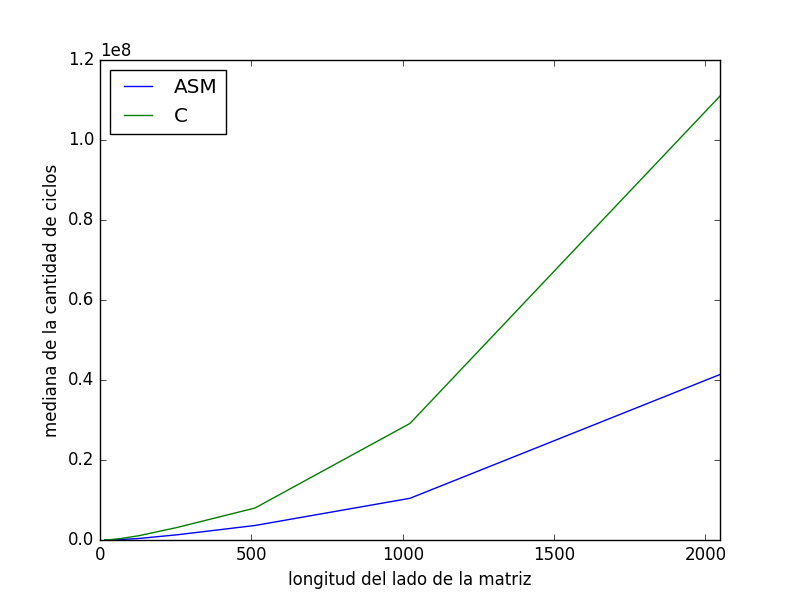
\includegraphics[width=12.5cm, height=9
cm]{images/car_tresColores.png}
\end{center}
\vspace{6px}


Como podemos observar la diferencia entre ASM y C es notoria. Esto se debe al paralelismo que se maneja en las instrucciones de SSE que se propuso utilizar en este trabajo. 

\subsection{Efecto Bayer}

La segunda experimentación que se realizó fue con el filtro de $Efecto$ $Bayer$, este mismo filtro deja solo uno de los 3 colores representantes de los píxeles con un patrón determinado. Como primera idea de las posibles mejoras que surgen a partir de utilizar ASM en vez de C, son los accesos a memoria. En general la cantidad de accesos a memoria se reduce, ya que trabajamos con múltiples píxeles al mismo tiempo. Este filtro no es la excepción y al traer de memoria 4 píxeles en vez de 1, como se haría con C, se mejoran mucho los tiempos. Continuemos con los resultados:


\vspace{6px}
\begin{center}
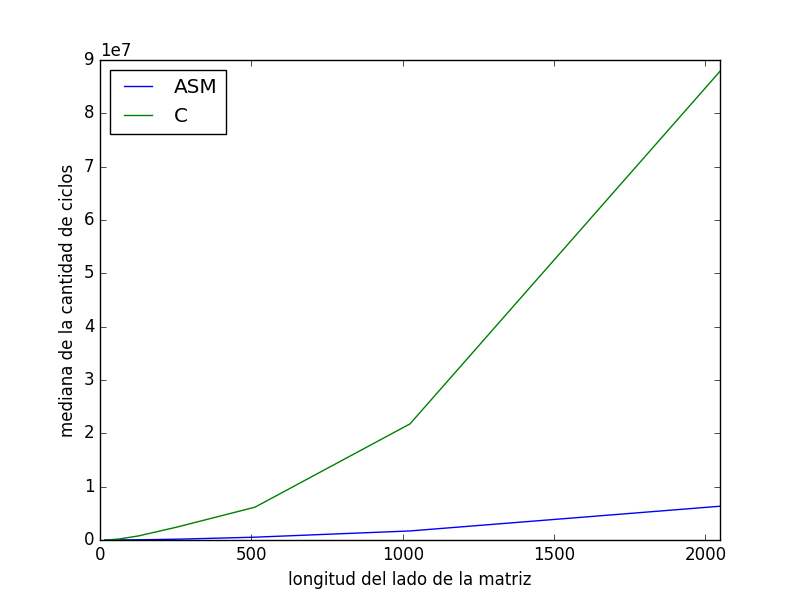
\includegraphics[width=12.5cm, height=9
cm]{images/car_efectoBayer.png}
\end{center}
\vspace{6px}

Podemos observar como el cambio es bastante alto con respecto a la implementación en C. Esto se debe, principalmente, a los accesos a memoria. Sin embargo, las operaciones que realizan las instrucciones de SSE influyen en los cambios de tiempo ya que se realizan simultáneamente.



\subsection{Edge Sobel}

La cantidad de operaciones que se realizan sobre en este filtro es bastante más que las que venimos trabajando anteriormente, por lo que uno de los posibles cambios en comparación con C, es que en ASM va a mejorar bastante el tiempo.


\vspace{6px}
\begin{center}
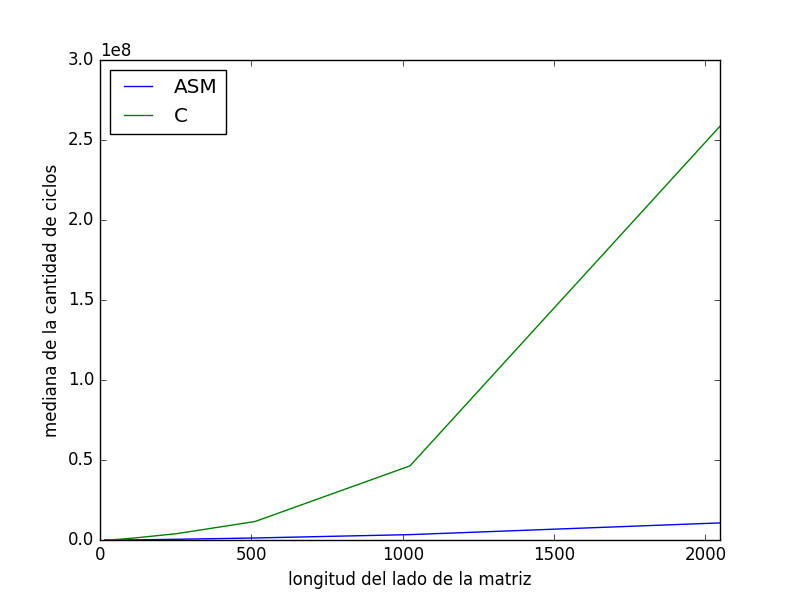
\includegraphics[width=12.5cm, height=9
cm]{images/car_edgeSobel.png}
\end{center}
\vspace{6px}





\subsection{Cambia Color}

En el caso de $Cambia$ $Color$ esperamos un cambio considerable ya que los accesos a memoria que se realizan dentro de cada iteración son 2, uno para traer los datos y otro para escribir. 

\vspace{6px}
\begin{center}
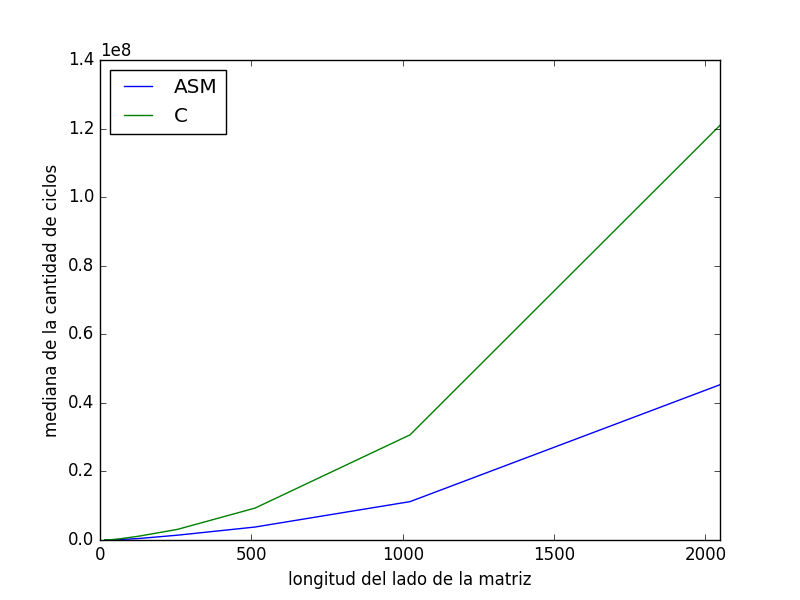
\includegraphics[width=12.5cm, height=9
cm]{images/car_cambiaColor.png}
\end{center}
\vspace{6px}

Podemos ver que el cambio es considerable, aunque no tanto como en otros filtros. Luego de un análisis se llegó a la conclusión de que el cambio de tiempos es bueno, aunque no mejor que otros filtros, debido a la cantidad de operaciones que tiene una iteración a comparación de los demás filtros. 